% Chapter Template

\chapter{Background} % Main chapter title

\label{c:background} % Change X to a consecutive number; for referencing this chapter elsewhere, use \ref{ChapterX}


	This chapter presents relevant background information on several topics for this thesis. 
	First, Section~\ref{s:mixedcriticality} reviews \emph{mixed criticality} and the scheduling theory which is the basis for Chapter~\ref{c:prof}. 
	Section~\ref{s:odr} reviews \emph{on-demand redundancy}, a type of error detection technique geared towards mixed criticality systems with fault-tolerance requirements. 
	Sections~\ref{s:nios} and \ref{s:hd} more specifically reviews the target platform for code generation and how \emph{fingerprinting} is used to detect errors to achieve on-demand redundancy.
	Section~\ref{s:ovp} reviews the virtual modeling tools used to develop software for the target platform.
	Section~\ref{s:simulink} discusses Simulink and the limitations imposed on Simulink generated code for the work in this thesis.
	
%----------------------------------------------------------------------------------------
%	SECTION 1
%----------------------------------------------------------------------------------------

\section{Mixed Criticality}
\label{s:mixedcriticality}
	Mixed criticality systems share resources between safety-critical tasks where failure can result in expensive damange or harm to users (e.g. x-by-wire), and non-safety critical tasks (e.g. infotainment). 
	Many industries such as automotive and avionics are trying to integrate low criticality (LO) and high criticality (HI) tasks onto the same processors.
	Mixed criticality scheduling (MCS) is the analysis of scheduling algorithms that provide safety guarantees to HI tasks in the presence of LO tasks \cite{burns2013mixed}.
	
	Adaptive mixed criticality (AMC), and more specifically the response time bound analysis (AMC-rtb) \cite{baruah2011response} is the baseline for much work in MCS. 
	AMC models applications as a set of as independent periodic tasks with fixed deadlines and periods (often assumed to be the same).
	Furthermore, HI tasks are assigned an optimistic and pessimistic worst case execution time (WCET). 
	The system is initially in a LO mode, where all tasks meet their deadline as long as they respect their optimistic execution time.
	Runtime mechanisms are put in place that detect when a task has exceeded its budget.
	In this case, the system transitions into the HI mode and drops as many LO tasks as necessary to guarantee that all HI tasks still have enough time to meet their deadlines provided their pessimistic execution times. 
	
	The formal notation for AMC is:
	\begin{itemize}
	  \item $\tau_i$: task $i$
	  \item $C_i(LO)$: LO mode WCET of $\tau_i$
	  \item $C_i(HI)$: HI mode WCET of $\tau_i$
	  \item $L_i$: Criticality of $\tau_i$ (LO or HI)
	  \item $T$: Period of $\tau_i$
	  \item $R_i$: Response time of $\tau_i$
	\end{itemize}

	Rate-monotonic scheduling assigns the highest priority to the task with the smallest period. Criticality inversion, depicted in Figure~\ref{f:responsetime}, is when LO tasks are able to preempt HI tasks. Priority inversion is desirable in mixed criticality systems if LO tasks have shorter periods than HI tasks \cite{baruah2011response}. However, this necessitates the runtime monitoring and mode change in case the effects of LO tasks risk causing a HI task to miss a deadline.

\addfigure{0.7}{responsetime.pdf}{Example of priority inversion in mixed criticality system using rate monotonic scheduling.}{f:responsetime}

AMC-rtb analysis consists of two equations for the response time of each task in the LO and HI mode:
\begin{equation}
R_i^{(LO)}= C_i(LO)+\sum_{j \in hp(i)}\Big\lceil\frac{R_i^{(LO)}}{T_j}\Big\rceil \cdot C_j(LO)
\label{eq:mode1}
\end{equation}
\begin{equation}
\begin{aligned}
R_i^{(HI)} &  = C_i(HI)+\sum_{j \in hpH(i)}\Big\lceil\frac{R_i^{(HI)}}{T_j}\Big\rceil \cdot C_j(HI) \\
&  +\sum_{k \in hpL(i)}\Big\lceil\frac{R_i^{(LO)}}{T_k}\Big\rceil \cdot C_k(LO)
\end{aligned}
\label{eq:mode2}
\end{equation}
where $hp(i)$ is the set of tasks with higher priority than $\tau_i$, $hpH(i)$ is the set of tasks with higher priority than $\tau_i$ that continue to execute in the HI mode, and $hpL(i)$ is the set of tasks with higher priority than $\tau_i$ that only execute in the LO mode.

	Equation~\ref{eq:mode1} defines the response time $R_i$ to be the LO mode WCET $C_i(LO)$ in addition to the worst-case amount of time all higher priority tasks $hp(i)$ may preempt $\tau_i$. 
	Equation~\ref{eq:mode2} shows that in the HI mode, the response time takes into account preemptions of $hpH(i)$ that are assumed to run for their pessimistic $C_i(HI)$. 
	Dropped tasks ($hpL(i)$) may still have preempted $\tau_i$ prior to the mode change and the third term in Equation~\ref{eq:mode2} models the carry-over effects.

% \section{Transient Faults}


\section{On-Demand Redundancy}
\label{s:odr}

	Transient faults or soft errors occur when environmental radation causes voltage spikes in digital circuits \cite{Baumann:05}. 
	Transient faults must be accounted for in safety critical applications despite their rare occurence due to the catastrophic consequences that may occur such as loss of life.
	All references to faults in this thesis refer only to transient faults whether or not explicitly stated. 
	This thesis is specifically focused on transient faults in the register files of processors. 
	Network \cite{radetzki2013methods} and memory \cite{Baumann:05} are also susceptible to transient faults however they are assumed to be dealt with by other mechanisms.


% 	Current solutions to transient errors typically rely on replication of entire boards. 
	Lockstep execution \cite{baleani2003fault} is the de-facto method of error detection in ECUs \cite{infineon2014aurix,freescale2014qorivva,renesas2016lockstep}. Lockstep execution, shown in Figure~\ref{f:lockstep}, consists of two cores executing the same code in parallel. 
	Lockstep implements redundancy at a very fine granularity as each store instruction is compared in hardware before being released to the bus. 
	If the store output does not match then some rollback procedure must be implemented or else the processors are restarted. 
	It is only possible to detect an error with two processors. 
	Correction can be implemented with three processors by majority vote. 
	Lockstep cores are difficult to build and scale due to the precise synchronization required.

	Lockstep execution is problematic in mixed criticality systems because it is not possible to \emph{decouple} the cores (i.e. use them to run different code independently). 
	It is inefficent to run mixed criticality applications on a pair of \emph{statically coupled} lockstep cores because not all tasks necessarily require protection against transient faults. 
	In Figure~\ref{f:lockstep}, both non-critical tasks (blue) as well as critical tasks (red) must execute on two cores at all times. 	
	The four physical cores operate as two logical nodes regardless of the workload.

	On-Demand redundancy (ODR) \cite{Meyer:CASES11,fu2013demand}, or dynamic core coupling \cite{lafrieda2007utilizing}, proposes the \emph{dynamic} coupling of cores in the system. 
	Only high criticality tasks requiring error detection will use two processors to execute redundant threads. 
	Figure~\ref{f:odr} shows how LO tasks are no longer forced to execute on two cores, thus freeing up resources to execute more tasks on the same number of cores.


\begin{figure}
\captionsetup[subfigure]{singlelinecheck=false}
\centering
\subcaptionbox{Lockstep execution \label{f:lockstep}}[0.45\textwidth]
{
    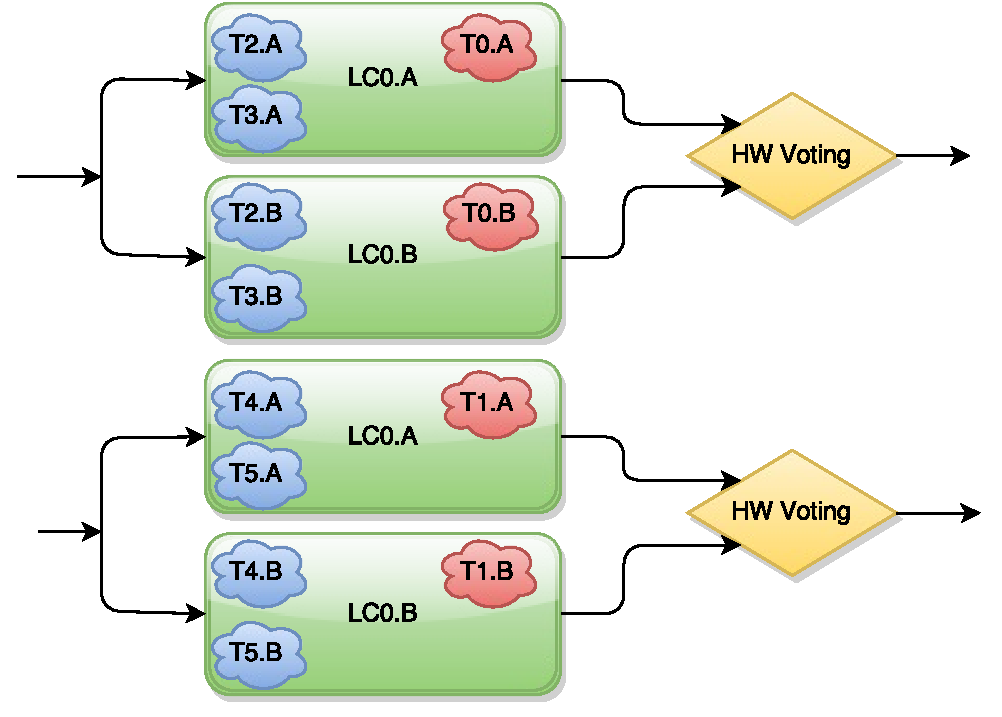
\includegraphics[width=0.42\textwidth]{lockstep.pdf}
}%
\hfill
\subcaptionbox[]{On-demand redundancy \label{f:odr}}[0.45\textwidth]
{
    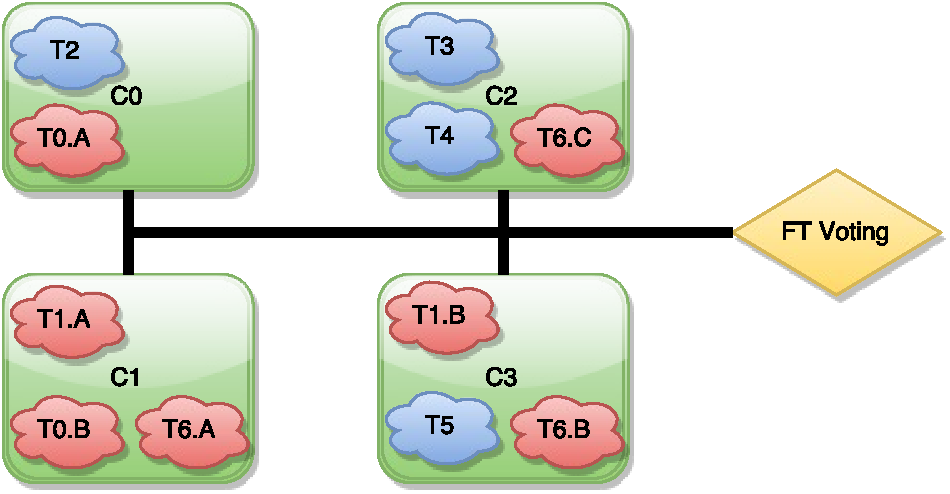
\includegraphics[width=0.42\textwidth]{odr.pdf}
}%
\caption[Short Caption]{Different architectures for multicore fault-tolerant systems.}
\label{f:ft-arch}
\end{figure}


\subsection{Fingerprinting with Nios Cores}
\label{s:nios}
	The target architecture is shown in Figure~\ref{f:platform-arch}. 
	A working FPGA prototype has been implemented with Nios II cores in previous work~\cite{ugthesis}. 
	The platform provides a mix of hardened cores and unreliable processing cores. 
	The goal of the platform is to explore the intersection of scheduling theory and a real-life implementation of on-demand redundancy. 
	In a real system at least one core would need to be fault tolerant to form a reliable computing base for the rest of the platform because thread level redundancy cannot catch errors in OS kernel code since it is not replicated \cite{dobel2012watches}. 
	The reliable monitor must be present to take more drastic correction measures (e.g. core reboot) in case the kernel itself is corrupted on any core.
	However, our FPGA prototype does not implement any specific fault tolerance mechanisms as we are concerned with higher level software design and resource management problems. 
	It is sufficient for these purpose to assume one of the cores has internal hardware mechanisms that increase its reliability.


\addfigure{0.6}{arch.pdf}{Platform Architecture}{f:platform-arch}

	ODR is implemented using fingerprinting \cite{Smolens:04} to detect errors. 
	The fingerprint hardware (FP) passively monitors bus traffic and generates checksums based on the write address and data.
	The software on each core signals the start, end, and pausing of a task to the FP unit.
	The hardware supports rate-monotic scheduling, meaning that a fingerprinted task may be paused and a higher priority task can begin fingerprinting without corrupting the previous fingerprint.
	Preemption is supported using modified exception funnels and stacks inside the FP however the implementation details were the subject of previous work \cite{ugthesis} and will not be discussed in this thesis.
	
	The sphere of replication (SoR) or fault containment region (FCR) refers to the notion that faulty data must not be allowed to propagate to main memory or I/O. 
	The fault tolerant core (FTC) maintains the SoR by moving temporary copies of critical data into the local scratchpad memory (SPM) of each processing core using DMA. 
	The processing cores are then notified to begin execution once the data is prepared. 
	The output of redundant tasks are not directly compared.
	Rather, the fingerprints are compared by an additional comparator hardware module and the results are forwarded back to the FTC. 
	When a task is successful, the FTC copies the data from one of the scratchpads back to main memory.
	
	The execution of redundant threads must be completely deterministic to generate identical fingerprints. 
	For instance, the uTLB implements virtual memory to allow the stack starting addresses and data locations must be identical on both copies for all store addresses to match.
% 	This is achieved using a virtual memory scheme using the uTLB.
	%All functions must take the location of global data as arguments in order to have matching stack references for both cores (Simulink provides this option by choosing reusable function interfaces).

\subsection{Fingerprints and Hamming Distance}
\label{s:hd}
	It must be decided when using fingerprinting how much state to compress into a single fingerprint. The larger the message being compressed, the more likely that \emph{aliasing} may occur, where the faulty fingerprint matches the correct fingerprint. 
	When using CRC, which is a modulo division operation, the likelihood of aliasing for a 32 bit divisor (or generator polynomial) converges to $2^{-32}$ \cite{Maxino:09}.
	
	The Hamming distance (HD) is the number of bits which are different between the faulty message and the correct message. 
	Certain 32 bit polynomials guarantee the absence of aliasing up to HDs of 5 or 6 if the message length is kept fairly small (under 32 kbits) \cite{koopman200232}.
	The argument for short fingerprinting intervals includes minimizing detection latency and decreasing the probability of aliasing.

	This implementation uses architectural fingerprinting as opposed to micro-architectural fingerprinting, meaning that the fingerprinting logic has not been integrated into the CPU and does not fingerprint micro-architectural state such as the register file or pipeline registers \cite{jared2007fingerprinting}.
	We also replicate and restore data at the granularity of a single task execution and are only concerned with the worst case timing.
	Only one fingerprint is necessary per task per period because enough resources must be allocated to handle the worst case latency (which occurs when a task fails near the end of its execution). 
		
	Figures~\ref{f:qsort-d} and \ref{f:qsort} show the average hamming distance (HD) and cumulative HD respectively for the qsort benchmark from the MiBench suite~\cite{guthaus2001mibench}. 
	The results were previously compiled using one and two bit fault injection on an instruction accurate simulation of the PowerPC architecture \cite{georgi}. 
	The figures show that the majority of errors with HD less than 10 bits are 1 or 2 bit errors and that the majority of errors result in HDs over 100. 
	We argue that aliasing should not be considered a critical design point since register errors either tend not to propagate or propagate well past the point where lower block sizes can decrease the likelihood of aliasing \cite{Maxino:09}.
	
	
	
\begin{figure}
% \captionsetup[subfigure]{}
\centering
\subcaptionbox{Average HD frequency \label{f:qsort-d}}[0.45\textwidth]
{	
    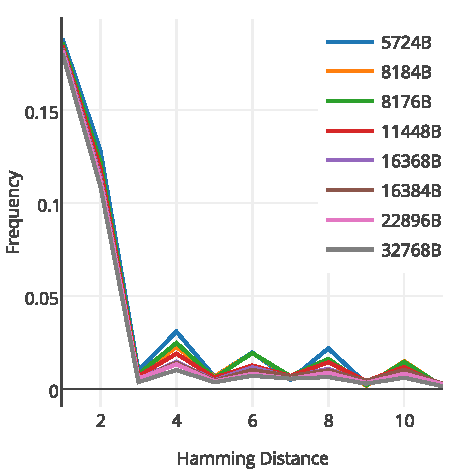
\includegraphics[width=0.45\textwidth]{qsort_d.pdf}
}%
\hfill
\subcaptionbox[]{Cumulative HD frequency \label{f:qsort}}[0.45\textwidth]
{
    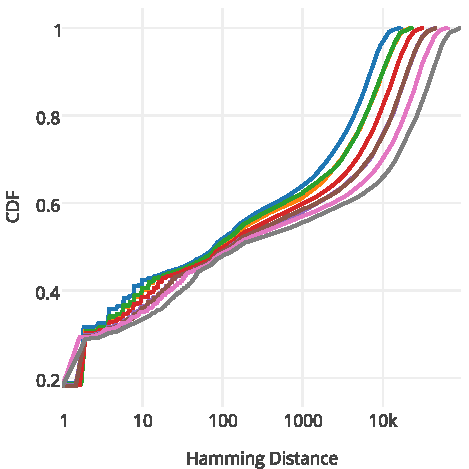
\includegraphics[width=0.45\textwidth]{qsort_nolegend.pdf}
}%
\caption{Fault injection results for qsort on PowerPC architecture}
\label{f:ft-arch}
\end{figure}

\section{Virtual Platform Model}
\label{s:ovp}
	This thesis is primarily concerned with the design and automatic generation of mixed-criticality software that runs on the proposed architecture. 
	All development, validation, and testing is done on a virtual model of the platform using Imperas simulation tools \cite{imperas} built on the Open Virtual Platform (OVP) instruction accurate simulation environment \cite{ovp}. 
	The purpose of developing on the virtual platform is to eventually validate the system on the FPGA implementation, however, software
	calibration on the FPGA is beyond the scope of this thesis.

\section{Simulink and Code Generation}
\label{s:simulink}
	Simulink is a dataflow language used to generate system models and control algorithms which provides the ability to export control algorithms as C code \cite{simulink}. 
	Simulink does not currently support multicore target platforms or fault tolerance. 
	The current state of the embedded runtime environment and assumptions made in the schedulability analysis places some severe limitations on the Simulink generated code supported by the framework presented in this thesis, namely:
\begin{itemize}
  \item The stack and heap requirements of any function cannot exceed 4kB (note that this limit could be increased but that \emph{some} hard limit must exist).
  \item There is no dataflow between tasks.
  \item Code is not generated to send results off-chip (e.g. sending results to actuators via IO).
\end{itemize}



